\documentclass[a4paper, 11pt, oneside]{article}

\usepackage[utf8]{inputenc}
\usepackage[T1]{fontenc}
\usepackage[english]{babel}
\usepackage{array}
\usepackage{shortvrb}
\usepackage{listings}
\usepackage[fleqn]{amsmath}
\usepackage{amsfonts}
\usepackage{fullpage}
\usepackage{enumerate}
\usepackage{graphicx}
\usepackage{alltt}
\usepackage{indentfirst}
\usepackage{eurosym}
\usepackage{titlesec, blindtext, color}
\usepackage[table,xcdraw,dvipsnames]{xcolor}
\usepackage[unicode]{hyperref}
\usepackage{url}
\usepackage{float}
\usepackage{subcaption}
\usepackage[skip=1ex]{caption}
\usepackage{dsfont}

\definecolor{brightpink}{rgb}{1.0, 0.0, 0.5}

\usepackage{titling}
\renewcommand\maketitlehooka{\null\mbox{}\vfill}
\renewcommand\maketitlehookd{\vfill\null}

\newcommand{\ClassName}{ELEN-0062: Introduction to Machine Learning}
\newcommand{\ProjectName}{Project 3 - Human Activity Prediction}
\newcommand{\AcademicYear}{2021 - 2022}

%%%% First page settings %%%%

\title{\ClassName\\\vspace*{0.8cm}\ProjectName\vspace{1cm}}
\author{Maxime Goffart \\180521 \and Olivier Joris\\182113}
\date{\vspace{1cm}Academic year \AcademicYear}

\begin{document}

%%% First page %%%
\begin{titlingpage}
{\let\newpage\relax\maketitle}
\end{titlingpage}

\thispagestyle{empty}
\newpage

%%%%%%%%%%%%%%%%%%%%%%%%%%%%%%%%%%%%%%%%%%

%%% Table of contents %%%
\tableofcontents
\newpage

%%%%%%%%%%%%%%%%%%%%%%%%%%%%%%%%%%%%%%%%%%

\section{Introduction}
\paragraph{}In this report, we will present and justify the different techniques we used for the third project of the course. The goal is to provide the reasoning behind our choices and to present the results obtained on Kaggle.

\section{Data pre-processing}
\paragraph{}We started by analyzing the data in order to pre-process them. Indeed, pre-processing is important
to have a good results when doing classification. This section includes the observations we made about the dataset
and different approaches we tried to solve the problems linked to this dataset.

\subsection{Filling missing values}
\paragraph{}The learning set contained a certain number of missing values represented by the \texttt{-999999.99} value. We thus started by looking at several 
methods proposed by the scikit-learn library\footnote{\url{https://scikit-learn.org/stable/modules/impute.html}}. We tried several of these methods and finally decided to use the \texttt{KNNImputer} which completes missing values using k-nearest neighbors : each missing value is imputed using the mean value from the nearest neighbors found in the training set. 

\subsection{Feature selection}

\begin{center}
    \begin{minipage}{0.5\linewidth}
    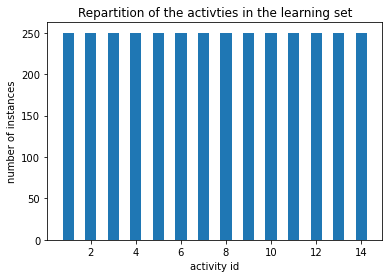
\includegraphics[width=\linewidth]{preprocessing/activity_repartition.png}
    \end{minipage}%
    \begin{minipage}{0.5\linewidth}
    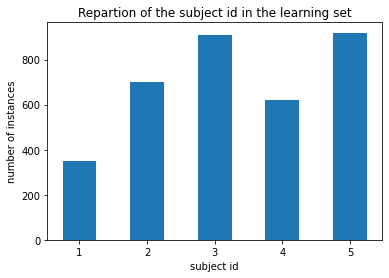
\includegraphics[width=\linewidth]{preprocessing/subjects_repartition.png}

    \end{minipage}
\end{center}

\paragraph{}We observed that the learning set seems to be balanced. We can see on the figure at the top right that the activity ID's are well distributed : they are each composed of 250 instances of the training set. However, when looking at the subject ID's of the learning set, we observed that some subjects have been less used to perform measures. This can be observed on the figure at the top right.
This can lead to overfit: all subjects have not the same behavior when perfoming an activity and the sensors measures are correlated to one subject.

\paragraph{}These observations and the fact that the dataset was really huge (3500 * 31 * 512 values), motivated us to perform features selection. We decided to perform feature selection using \texttt{SelectFromModel}\footnote{\url{https://scikit-learn.org/stable/modules/feature_selection.html}}. It is perfoming ranking based on one estimator and then remove the less ranked features recursively. We chose the \texttt{ExtraTreeClassifier}\footnote{\url{https://www.geeksforgeeks.org/ml-extra-tree-classifier-for-feature-selection/}} as estimator for this method. It is similiar to a random tree classifier and only differ in the manner it is constructed which lead to the creation of multiple de-correlated decision trees. This seems us to be a good model to rank the features because we have seen in the theoritical course that decision trees are nice to discriminate features but are too much related to the dataset. It is why the way the Extremely Randomized Trees are constructed reduce the variance link to the dataset and thus reduce the chances of overfitting.

\subsection{Implementation}

The implementation of this part can be found in the \texttt{preprocessing.ipynb} notebook or in the \texttt{preprocessing.py} python script. We have performed some tests measuring the scores and it is a bit increasing the scores of our models.

\section{Studied models}

\subsection{K-nearest neighbors}
\paragraph{}First, we decided to use the K-nearest neighbors method because it was the one provided by the pedagogical team with the assignment. Yet, the reasons that made us trying multiple versions of this technique are the facts that it is easy to interpret and to use.

\subsubsection{1-NN} \label{1NN}
\paragraph{}Our first submission was the one provided with assignment\footnote{File \texttt{example\_submission.csv}.} that was generated with the 1-nearest neighbor model\footnote{Files \texttt{toy\_script.py} or \texttt{knn\_basic\_1.py}.}.\\
This submission yields a score of 0.52 on Kaggle.

\subsubsection{25-NN}
\paragraph{}Based on \ref{1NN}, we decided to increase the value of K of the K-nearest neighbors method to 25. The motivation behind the choice of this value for K was theoretical. Since the dataset is huge and can contain errors in the measured values, we though that increasing the value of K would increase the precision of the model because each prediction will not depend on a single neighbor that could have been misclassified.\\
This technique is implemented in the file \texttt{knn\_basic\_25.py}. This submission yields a score of 0.54 on Kaggle.

\subsubsection{55-NN and 49-NN}
\paragraph{}We decided to keep using the K-NN method to study how well it could perform on the assignment. We decided to study the accuracy of the KNN technique by using a 10-fold cross validation technique with the negative log loss function as a scoring measure. We obtained the following graph of accuracies depending on the value of K:
\begin{figure}[H]
\center
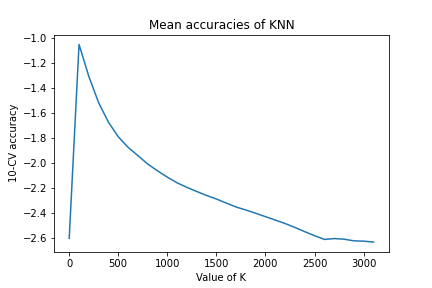
\includegraphics[scale=0.3]{knn/log_loss.png}
\caption{10-CV accuracy of KNN depending on value of K}
\end{figure}
We could see that there is a peak. By using a divide and conquer technique, we found that the peak was obtained for values of K around 50. Thus, we decided to study the accuracy in a small range of K values around $K=50$. We obtained the following graph:
\begin{figure}[H]
\center
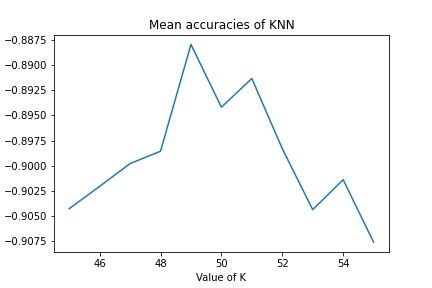
\includegraphics[scale=0.4]{knn/log_loss_focused.png}
\caption{10-CV accuracy of KNN depending on value of K}
\label{knn_log_loss_focused}
\end{figure}
\paragraph{}Based on the divide and conquer approach performed, we decided to use 55 neighbors. The choice of this value was motivated by the fact that we observed a peak around this value.\\
This submission yields a score of 0.53142 on Kaggle and the implementation of it is inside the file \texttt{knn\_basic\_55.py}.
\paragraph{}Then, based on the graph of figure \ref{knn_log_loss_focused}, we decided to use 49 neighbors. The choice of this value was motivated by the fact that it yields the highest score on the learning set by using a 10-fold cross validation strategy with the negative log loss function as a scoring measure.\\
This submission yields a score of 0.52571 on Kaggle which is less than the one for 55-NN. Yet, we expected a higher score based on the graph of figure \ref{knn_log_loss_focused}. The implementation is available inside the file \texttt{knn\_basic\_49.py}.
\paragraph{}Based on the two previous results, we came to the conclusion that using "vanilla" K-nearest neighbors was not sufficient. Thus, we decided to find new techniques explained in the following sections.

\subsubsection{Multiple K-nearest neighbors models} \label{knnMultiple}
\paragraph{}We took a look back at the slides provided with the assignment and we focused on the features (sensors) of the datasets. We noticed that the features are not in the same units. Thus, we thought about using multiple 1-nearest neighbor models with one 1-NN model per feature. This idea was motivated by the fact that we though we would obtained a better accuracy by using one 1-NN per feature because measurements in different units would not be mixed.\\
We implemented this approach in the file \texttt{knn\_splitted\_1.py}. This yields a score of 0.52 on Kaggle which is the same as the toy script provided with the assignment.

\subsubsection{Mutiple K-nearest neighbors models and samples modification}
\paragraph{}After the disappointing result obtained in \ref{knnMultiple}, we decided to take a better a look at the datasets. We noticed that some samples were vectors full of -999999.99. We though that these measurements would badly influenced the models. Thus, we decided to replace each sample that was a vector full of -999999.99 by a vector full of 0.\\
We implemented this approach in the file \texttt{knn\_splitted\_1\_filtered.py} and the score obtained on Kaggle was 0.53142.

\subsubsection{Conclusion on K-nearest neighbors}
\paragraph{}After all the different tries perform using K-nearest neighbors models, we came to the conclusion that "vanilla" K-NN were not sufficient for this project.\\
The codes for the different plots are available inside the Jupyter notebooks \texttt{knn\_basic.ipynb} and \texttt{knn\_splitted.ipynb}.

%%%%%%%%%%%%%%%%%%%%%%%%%%%%%%%%%%%%%%%%%%
\end{document}